\documentclass[11pt,letterpaper]{article}
\usepackage[lmargin=1in,rmargin=1in,tmargin=1in,bmargin=1in]{geometry}
\usepackage{../style/homework}
\usepackage{../style/commands}
\setbool{quotetype}{false} % True: Side; False: Under
\setbool{hideans}{true} % Student: True; Instructor: False

% -------------------
% Content
% -------------------
\begin{document}

\homework{2: Due 05/04}{All things are subject to interpretation. Whichever interpretation prevails at a given time is a function of power and not truth.}{Friedrich Nietzsche}

% Problem 1
\problem{10} A relation $f(x)$ is graphed on the plot below.
	\[
	\fbox{
	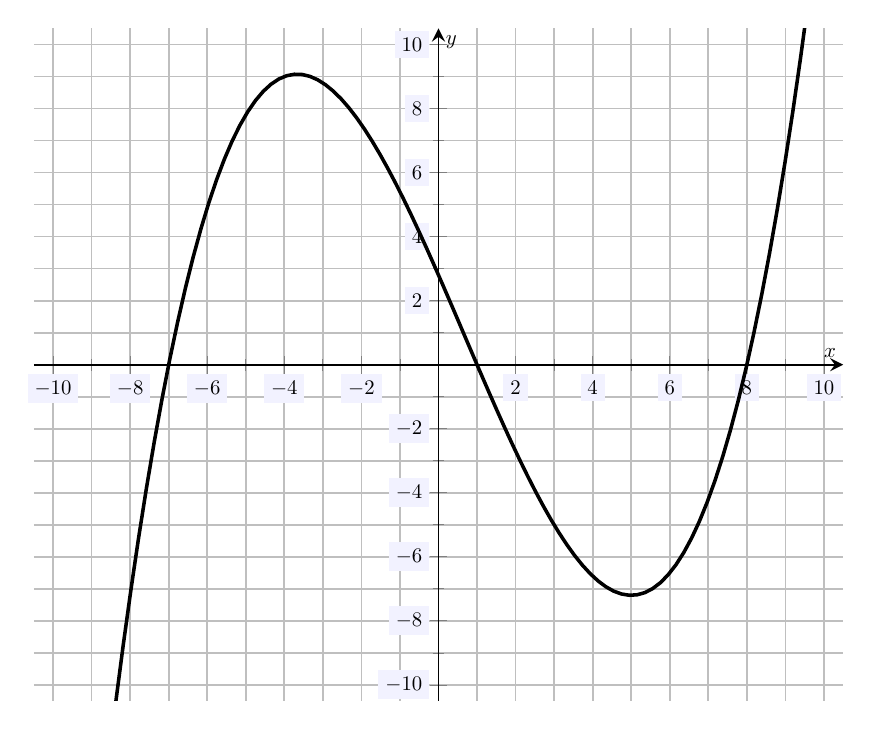
\begin{tikzpicture}[scale=1.5,every node/.style={scale=0.5}]
	\begin{axis}[
	grid=both,
	axis lines=middle,
	ticklabel style={fill=blue!5!white},
	xmin= -10.5, xmax=10.5,
	ymin= -10.5, ymax=10.5,
	xtick={-10,-8,...,10},
	ytick={-10,-8,...,10},
	minor x tick num = 1,
	minor y tick num = 1,
	xlabel=\(x\),ylabel=\(y\),
	]
	\node at (4.5,60) {\Large$R(q)$};
	\addplot[domain=-10:10,samples=100,line width=0.03cm] ({x}, {1/20*(x + 7)*(x - 1)*(x - 8)});

	\end{axis}
	\end{tikzpicture}
	}
	\] 

\begin{enumerate}[(a)]
\item Is the relation above a function? Explain. 
\item Does the relation above have an inverse function? Explain.
\end{enumerate}



\newpage



% Problem 2
\problem{10} A function $f(x)$ is plotted below. On the same plot, graph the function $g(x)= 4 - f(x - 5)$.
	\[
	\fbox{
	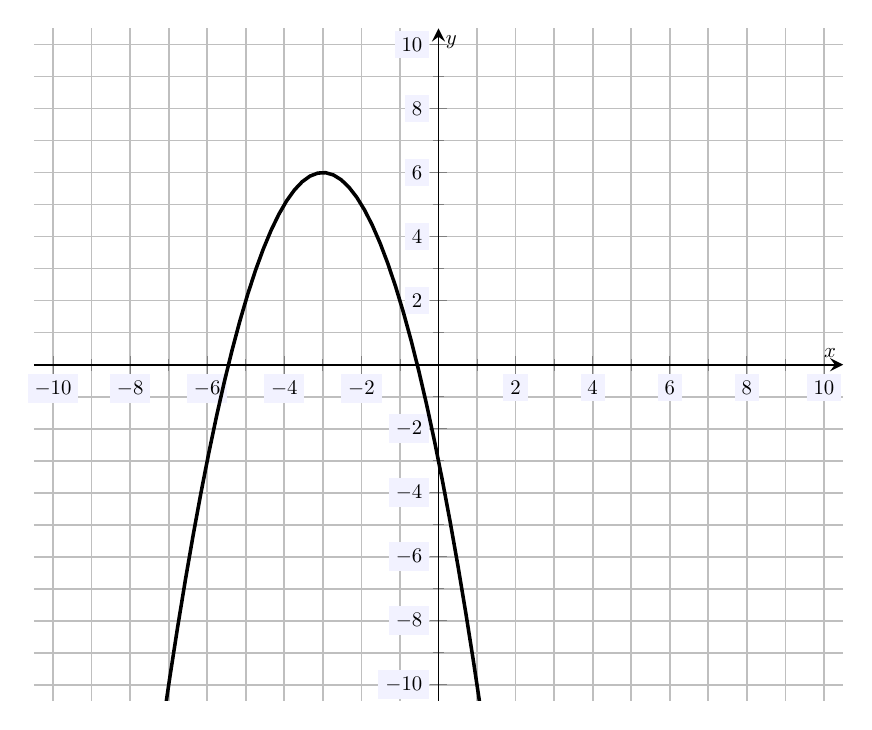
\begin{tikzpicture}[scale=1.5,every node/.style={scale=0.5}]
	\begin{axis}[
	grid=both,
	axis lines=middle,
	ticklabel style={fill=blue!5!white},
	xmin= -10.5, xmax=10.5,
	ymin= -10.5, ymax=10.5,
	xtick={-10,-8,...,10},
	ytick={-10,-8,...,10},
	minor x tick num = 1,
	minor y tick num = 1,
	xlabel=\(x\),ylabel=\(y\),
	]
	\node at (4.5,60) {\Large$R(q)$};
	\addplot[domain=-10:10,samples=100,line width=0.03cm] ({x}, {-x^2 - 6*x - 3});

	\end{axis}
	\end{tikzpicture}
	}
	\] 


\end{document}